\chapter{Implementation}

In this chapter, we present the implementation details of our proposed decisions. 

In order to achieve goals from ~\ref{sec:concept}, it is necessary to formulate technical requirements for implementation. After a thorough study of the literature \cite{buitinck2013api}, we put forward the following requirements:

\begin{itemize}
    \item \textbf{Components.} To meet the needs of flexible architecture, we need to divide the optimization workflow into logical steps and abstract them. These abstractions are interpreted as easily replaceable components. Only in the case of homogeneity of optimization processes with the standard interfaces, it is possible to scale the optimization approach to multi-objective tasks.
    \item \textbf{Separation of concerns.} In order to ensure more considerable optimization variability, it is necessary to evaluate the optimization steps independently.
    \item \textbf{Non-proliferation of classes.} To improve the compatibility of our solution with other frameworks, we need to use a simple structure to share information.
\end{itemize}

The following frameworks were used to fulfill the criteria.
\begin{description}
    \item \textbf{Scikit-learn} \cite{art-scikit-learn} is one of the most popular machine learning framework that accomplishes with a variety of learning tasks. The crucial features are excellent documentation and reusable components in various contexts. Extensibility and consistent interfaces resulted in large and active community of library. Scikit-learn integrates well with many other Python libraries. 
    \item \textbf{pygmo2} \cite{francesco_biscani_2019} is scientific library with an effective parallelization for local and global optimization. Key features of this project are efficient implementations of bio-inspired and evolutionary algorithms and unified interface to optimization algorithms and problem definitions. 
\end{description}


Next, specific optimization steps will be discussed.
% --------------------------------------------------------------------------------------------
% ---------------------------------------------------       Compositional surrogate      
% --------------------------------------------------------------------------------------------
\section{Compositional surrogate}

    The Composite Surrogate provides the ability to aggregate several simple models to promote multi-objective extrapolation.

    To achieve this goal, the Model-union class (Figure \ref{fig:munion}) class was implemented. It is implement \emph{a compositional design pattern} \cite{bookGOF} where several heterogeneous models could be combined. This class is as meta-model that wraps and aggregate surrogates and could be combined in a tree structure. Such an architectural solution is needed to improve the scalability of surrogates as components
    
    % % Note that Scikit-learn tends to use "duck typing", so building a model which supports require methods suffices for compatibility. Internal classes such as \textit{BaseEstimator} provide boilerplate code and is used for clarity and convenience intent.
    A parent class that combines multiple models can combine their approximations in several ways:
    \begin{itemize}
        \item \textbf{Stacking.} It is an ensemble approximation technique which average obtain results from each child model. The child regression models are trained based on the whole training samples. 
        \item \textbf{Split y.} A straightforward technique to combine several regression models in multi-label prediction case. Each child surrogate is trained on the entire dataset, including only one objective of interest. This functionality allows as to produce multi-objective compositional surrogate from combinations of single-objective models.

    \end{itemize}

    % ==== Sampling plan
    \begin{figure}
        \centering
        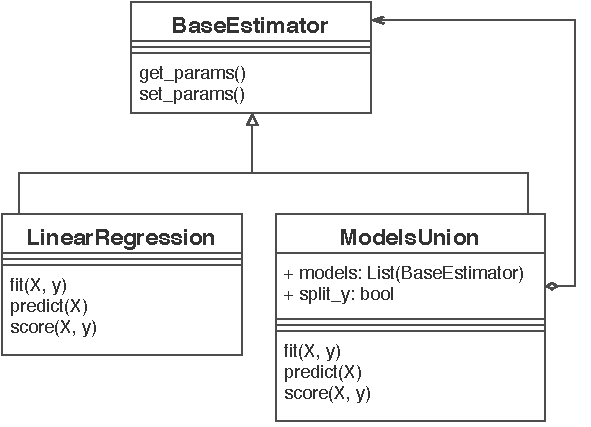
\includegraphics[width=10cm]{content/images/munion_class}
        \caption[Models-union class]{Class diagram of \textit{ModelsUnion}} 
        \label{fig:munion} 
    \end{figure}  

    So, Model-union class puts the compositional model on one line with other surrogate models. It allows us to independently validate many surrogate models and combine them in a surrogate portfolio.

% --------------------------------------------------------------------------------------------
% ---------------------------------------------------       Optimization orchestrator     
% --------------------------------------------------------------------------------------------
\section{Optimization orchestrator}
    The \textit{TutorModel} (TutotM) Class is the orchestrator of all optimization steps. TutorM is responsible for parallel surrogate build, their validation and combination. Also, TutorM provides surrogate models to the optimization algorithm. Due to the principle of separation of concerns, the surrogate model does no depend on the optimization technique. As a result, this extensive combination can provide additional flexibility and the ability to adapt to specific problems. An example of the workflow of TutorModel is presented in the Figure \ref{fig:tutor_activity}, As can we note, there are three surrogate models in the portfolio, from which pass validation only two.
    
    Validation is the primary source of information for deciding on a surrogate model.


        % ==== Figure
        \begin{figure}[h]
            \centering
            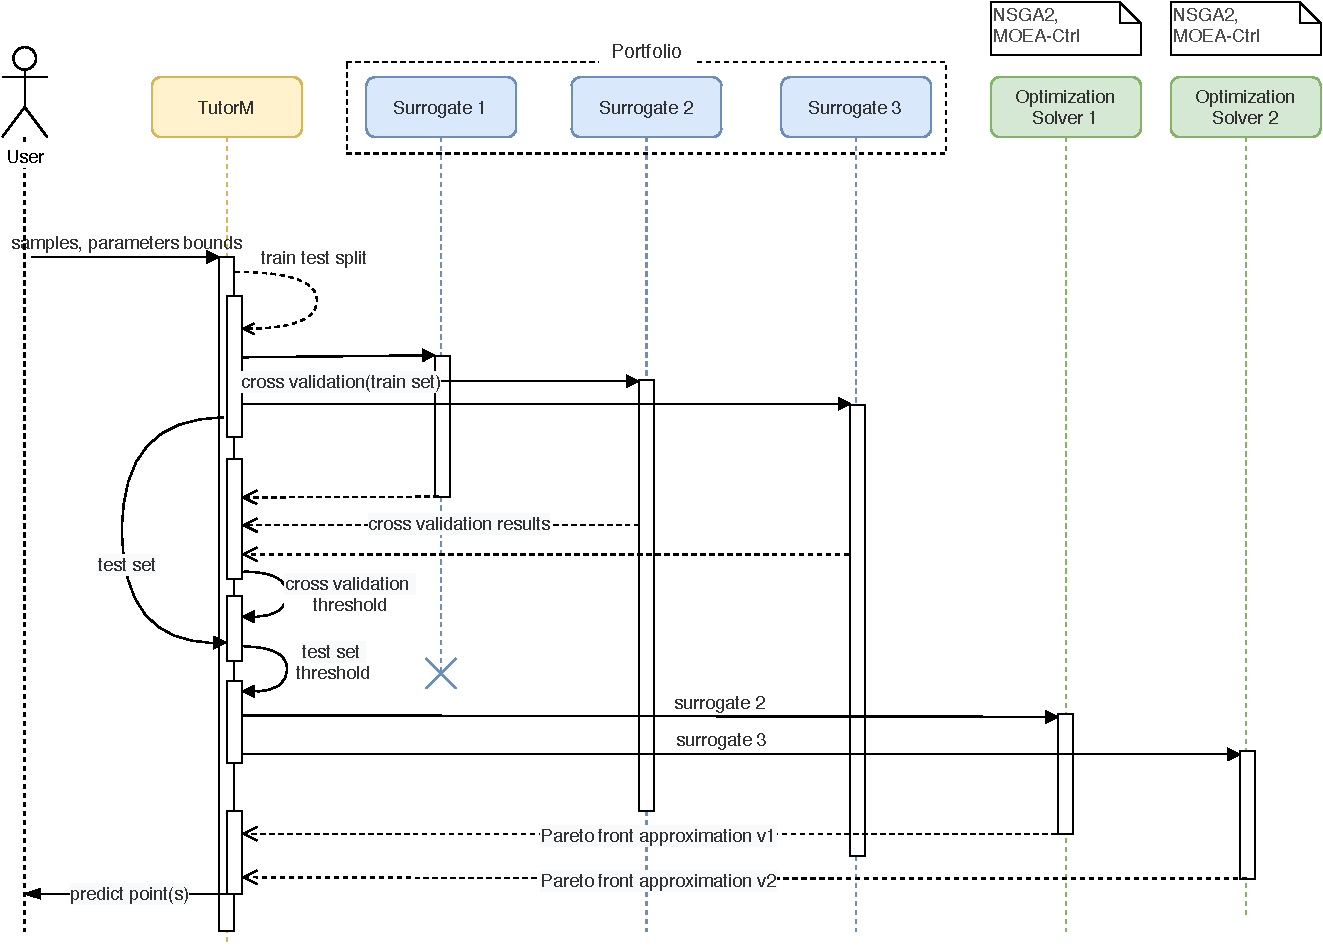
\includegraphics[width=\textwidth]{content/images/portfolio_validation_solv}
            \caption[Portfolio validation activity]{Optimization iteration with three surrogate models and two optimizers}
            \label{fig:tutor_activity}
        \end{figure}

    % ---------------------------------------------------        Validation
    \paragraph{Surrogates validation}
        To select a surrogate model, we need to check the accuracy of the assumption from unknown experiments(test set). As mentioned early Chapter~\ref{sec:concept}, validation should be done in several stages to avoid overfitting (Figure \ref{fig:simsim_activity_validation}). The validation steps are as follows: At the first stage, models are selected based on \emph{cross validation} technique. In this stage define lower bound for overall accuracy. We notice that pass this threshold does not guarantee that surrogate is useful. 2) On the last stage, valid models from the previous stage are evaluated and selected for optimization.

            % ==== activity_validation
            \begin{figure}
                \centering
                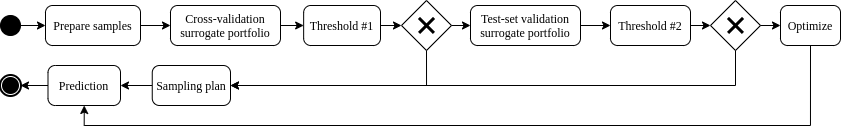
\includegraphics[width=\textwidth]{content/images/simsim_activity_workflow}
                \caption[General workflow activity]{General optimization workflow for model-based optimization iteration with validation in two stages.}
                \label{fig:simsim_activity_validation}
            \end{figure}

    \paragraph{Optimization algorithm}
        The role of the optimization algorithm is to find a near-optimal solution based on surrogate approximation. While other methods also exist, we select \gls{moea} as the main solver because it can be applied to a wide range of problems. 
       
        Optimization framework requires the definition of custom problems. The optimization problem is not built on top of surrogate models, but are used with the help of surrogate models. In the case of the genetic algorithm, it produces the population of parameters, that could be treated as a Pareto front approximation. If several surrogates are valid than several Pareto front approximations obtain. There are two approaches to select the most informative solutions: 1) pick Pareto approximation from surrogate with the highest accuracy in non-dominated points. 2) Assume that all approximations are valid and all points could be selected. In this case, intersection predictions from samples have a higher probability of being selected. 
        

    % ---------------------------------------------------        Portfolio        
    \paragraph{Surrogate portfolio}
    Since the surrogate model can produce different results on a different problem, it is necessary to choose a model from the portfolio.

    Surrogate models can be divided into two groups: a multi-output model for all objectives and compositional model with single-output models. All models pass validation equally, but after cross-validation single-objective models should combine with another one to provide multi-objective surrogate hypothesis. During this process, all objectives should be restored from valid surrogates. 




    \section*{Conclusion} 
    
    We implemented a base class that can deal with a composite surrogate model and can combine arbitrary model to apply for a multi-criteria problem. The TutorM class is required to bring together implemented features such as surrogate portfolio, validation strategy and dynamic compositional model. Also, the requirements for the implementation of the proposed strategy have been identified. Mentioned requirements are intended to improve the further support and benefits of the developed method.


        
    % % ---------------------------------------------------        Sampling strategy
    % \paragraph{Sampling strategy} In many practical problems, only a restricted budget is spendable. Each evaluated point should be informative to reduce cost and improve interpolation by models. The most straightforward method of sampling design is a random which for small sample sizes, that often produce clusters of samples. Conversely, there are also quasi-random distributions that produce informative samples that cover space more evenly. Most popular algoruthms are Sobol\cite{Sobol1999} and Latin hypercube sampling.


% --------------------------------------------------------------------------------------------
% ---------------------------------------------------       Solvers      
% --------------------------------------------------------------------------------------------

    % Optimization algorithms. MOEA. A Python platform\cite{francesco_biscani_2019}  to perform parallel computations of optimisation tasks (global and local) via the asynchronous generalized island model.

    % decorators for single-objective solver with multi-objective surrogate 








% ----------    Designing a Sampling Plan
% \paragraph{Designing a Sampling Plan} The most straightforward way of sampling a design space in a uniform fashion is by \cite{EngSurMod} means of a rectangular grid of points. 
% Random sampling has the downside that for small sample sizes, there is often signficant clustering of samples, which is not ideal for interpolation since clustered samples can be wasteful. Instead, often a better option is to use a Latin hypercube, which enforces a condition that sample bins may not share the same coordinates for any coordinate axis







% Without automated tools, it can take days for experts to review just a few dozen examples.  In that same time, an automatic tool can explore thousands to millions to billions more solutions. People find it an overwhelming task just to certify the correctness of conclusions generated from so many results.


% Managing complex execution Strategies


% The simplifications are mean to discard the superfluous details that are unlikely to generalize to new instances. However, to decide what data to discard and what data to keep, you must make a hypothesis. For example, a linear model makes the hypothesis that the data is fundamentally linear and that the distance between the instances and the straight line is just noise, which can safely be ignored.



% sklearn 'duck typing'. This means that estimators are defined by interface, not by inheritance, where the interface is entirely implicit as far as the programming language is concerned.

% Variants in the evaluation of sets of solutions for each hypothesis. Each hypothesis has quality metrics. Solution(s) from each hypothesis have also own metrics.


% Intuition of why random forest is a good model: •Good at non-linearity, multi-modality and non-smoothness. A decision tree is a non-parametric supervised machine learning method widely used to formalize decision making processes across a variety of fields. The combination of many weak regressors (binary decisions) allows approximating highly non-linear and multi-modal functions with great accuracy. In addition, random forests naturally deal with categorical and ordinal variables which are important in computer systems optimization.
